\appendix

\chapter{The InsightVLM Chart Tester}
\label{app:tester}

The tester is a local web application (\texttt{app.py}, built with Gradio) for trying the
model on any chart. It loads the deployed ensemble from
\texttt{results/final\_ensemble.json} and runs every input through exactly the pipeline
that produced the reported numbers: resize to $384\times384$, each member's softmax,
equal-weight average, and the (zero-strength) label-shift correction.

\begin{figure}[h]\centering
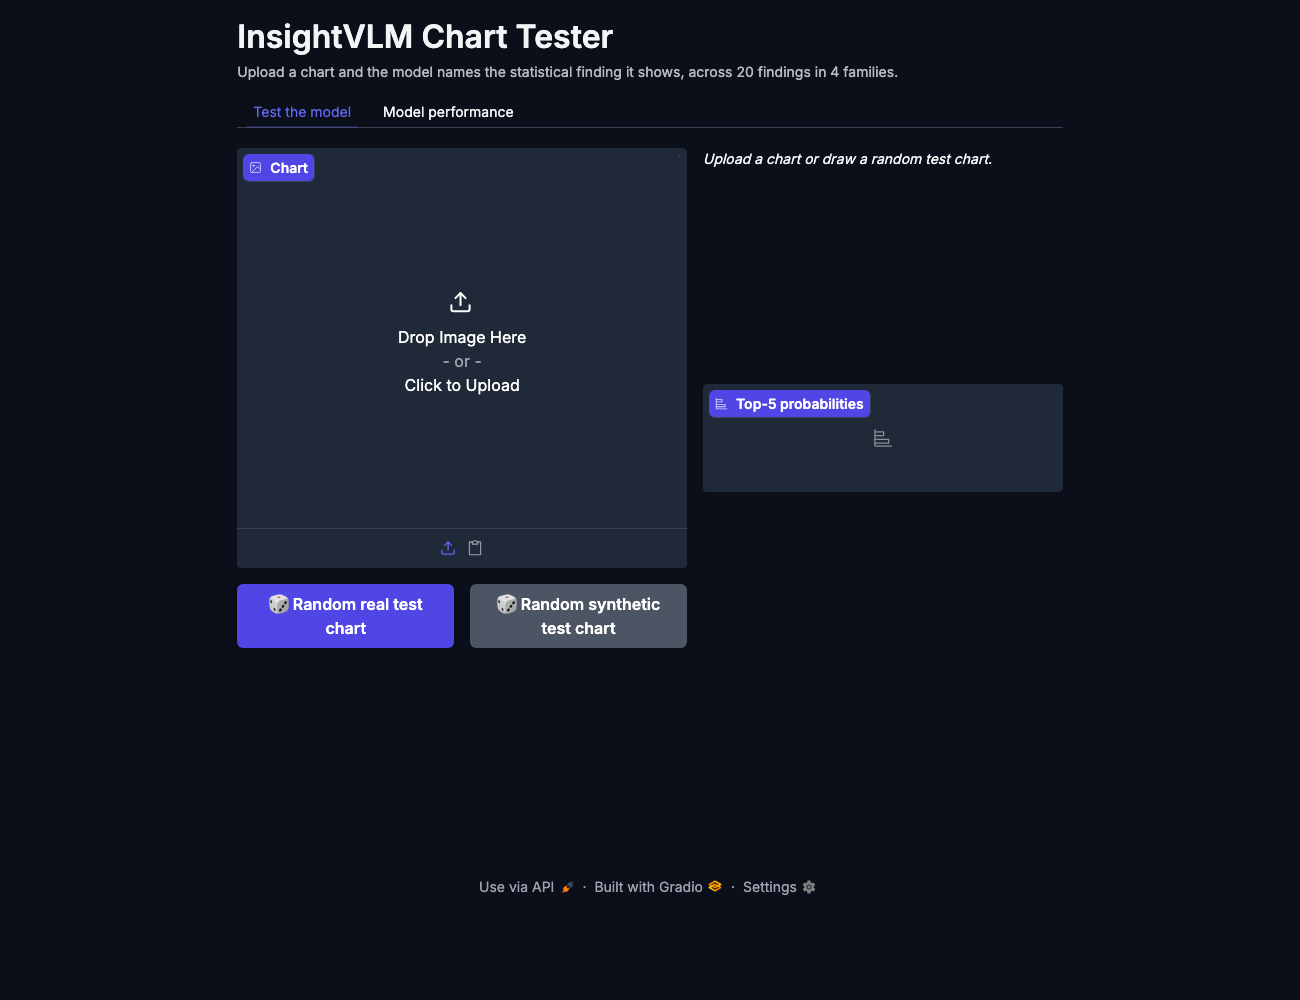
\includegraphics[width=0.85\linewidth]{app_home.png}
\caption{The tester's main tab. A chart can be uploaded, pasted from the clipboard, or
drawn at random from the held-out real or synthetic test charts.}
\label{fig:app}
\end{figure}

\paragraph{Running it.}
\begin{verbatim}
pip install torch torchvision gradio pandas pyarrow pillow
python app.py            # then open http://127.0.0.1:7860
\end{verbatim}

\paragraph{What it shows.} For an uploaded chart:
\begin{itemize}[leftmargin=1.3em]
  \item the predicted finding in plain language, its confidence, and its family;
  \item how many ensemble members agree;
  \item the definition of the finding and the statistical test that licenses it;
  \item the five most probable findings;
  \item a warning when confidence is below 50\%, since the chart may show a mix of
  patterns or one outside the 20 classes.
\end{itemize}
The \emph{random real test chart} and \emph{random synthetic test chart} buttons draw a
held-out test chart, predict it, and show the verified ground truth, its source, chart
type, difficulty and verified insight beside the prediction, marked correct or wrong.
The \emph{Model performance} tab lists the ensemble's test accuracy on real and synthetic
charts against the zero-shot baselines and the no-pixel floor.

\paragraph{Limits.} The tester classifies into the 20 known findings only. Charts from
tools unlike the training renderers are less reliable (Section~\ref{sec:rq4}), and
compound findings are reported as a single class.

\chapter{Artefacts and Reproduction}
\label{app:repro}

Every number in this thesis is produced by a script in the project repository
(Table~\ref{tab:repro}). Training ran on Kaggle (two T4 GPUs) from notebooks generated
by \texttt{train/make\_split\_notebooks.py}; everything else runs on a laptop CPU or
Apple-silicon GPU.

\begin{table}[h]\centering\small
\caption{Where each result comes from.}
\label{tab:repro}
\begin{tabular}{p{5.2cm}p{9.0cm}}
\toprule
\textbf{Result} & \textbf{Command or file} \\
\midrule
Dataset build and audit & \texttt{python run\_all.py}; \texttt{build/07\_validate.py}; \texttt{build/10\_bias\_audit.py} \\
Clean (version-2) renders & \texttt{build/06\_render.py --clean} \\
Supplementary real pool & \texttt{build/12\_extra\_real.py}, then \texttt{06\_render.py --records cache/records\_extra.jsonl} \\
Plotly / Vega-Lite test renders & \texttt{build/11\_render\_plotly.py}; \texttt{build/13\_render\_vega.py} \\
Augmentation renders & \texttt{11\_render\_plotly.py --split train}; \texttt{06\_render.py --randstyle} \\
Model training & notebooks \texttt{nb5\_real}, \texttt{nb5x\_*}, \texttt{nb7\_*} \\
Zero-shot VLM baselines & notebooks \texttt{nb6\_zeroshot}, \texttt{nb6b\_zeroshot\_ts} \\
Leak ablation (Table~\ref{tab:leak}) & \texttt{train/ablate\_marks.py} \\
Probabilities per model and renderer & \texttt{train/cache\_probs.py [--view plotly|vega]} \\
Deployed ensemble & \texttt{train/final\_ensemble.py} $\rightarrow$ \texttt{results/final\_ensemble.json} \\
Main table, CIs, McNemar & \texttt{train/stats\_report.py} $\rightarrow$ \texttt{results/stats\_report.json} \\
Grounding (Table~\ref{tab:grounding}) & \texttt{train/grounding\_eval.py} $\rightarrow$ \texttt{results/grounding.json} \\
Figures & \texttt{paper/make\_figures.py} \\
Human label check (Table~\ref{tab:labelcheck}) & \texttt{train/human\_study\_eval.py} (answers and key kept private) \\
\bottomrule
\end{tabular}
\end{table}

\paragraph{Data.} InsightVLM-20K version 2 is on Kaggle
(\texttt{asifxzaman/insightvlm-20k-v2}), with the supplementary pool
(\texttt{insightvlm-extra-real}) and the augmentation renders
(\texttt{insightvlm-aug-train}). The datasheet (\texttt{DATASHEET.md}) and audit report
(\texttt{BIAS\_AUDIT.md}) ship with the data.
